%
% File vlsp2020.tex
%
%% Based on the style files for ACL 2020, which were
%% Based on the style files for ACL 2018, NAACL 2018/19, which were
%% Based on the style files for ACL-2015, with some improvements
%%  taken from the NAACL-2016 style
%% Based on the style files for ACL-2014, which were, in turn,
%% based on ACL-2013, ACL-2012, ACL-2011, ACL-2010, ACL-IJCNLP-2009,
%% EACL-2009, IJCNLP-2008...
%% Based on the style files for EACL 2006 by 
%%e.agirre@ehu.es or Sergi.Balari@uab.es
%% and that of ACL 08 by Joakim Nivre and Noah Smith
%% Used as VLSP's template since Dec 2020, adapted by Xuan-Son Vu.

\documentclass[11pt,a4paper]{article}
\usepackage[hyperref]{acl2020}
\usepackage{times}
\usepackage{latexsym}

\usepackage{amssymb}
\usepackage{amsmath}
\usepackage{todonotes}
\usepackage{hyperref}
\usepackage[nowatermark]{fixmetodonotes}
\renewcommand{\UrlFont}{\ttfamily\small}
\renewcommand{\baselinestretch}{1.15} % giãn dòng
\usepackage{graphicx}
\graphicspath{ {./images/} }

% This is not strictly necessary, and may be commented out,
% but it will improve the layout of the manuscript,
% and will typically save some space.
\usepackage{microtype}

\aclfinalcopy % Uncomment this line for the final submission
%\def\aclpaperid{***} %  Enter the acl Paper ID here

%\setlength\titlebox{5cm}
% You can expand the titlebox if you need extra space
% to show all the authors. Please do not make the titlebox
% smaller than 5cm (the original size); we will check this
% in the camera-ready version and ask you to change it back.

\newcommand\BibTeX{B\textsc{ib}\TeX}
\title{Decision Support System Technical Report \\ 
Applying Regularized Linear Model in Predicting house price 
}
\author{~~NGUYEN Duc Thien ~~VU Hoang Duc Hieu ~~LE Duc Thang ~~TRINH Ngoc Khang ~~PHAM Van Hai\thanks{*Corresponding author} \\
  ~~~~~~~~~~~~~~~~~~~~School of Information and Communication Technology \\
  ~~~~~~~~~~~~~~~~~~~~Hanoi University of Science and Technology \\
  ~~~~~~~~~~~~~~Hanoi, Vietnam \\
}

\date{}

\begin{document}
\maketitle

\begin{abstract}

This paper presents our approaching model to solve the task of \emph{House Prices - Advanced Regression Techniques} which was public on \cite{kaggle}. We implemented the . Our model used ... to . Experiments on the test show that our model achieves 0.12299 Root Mean Square Logarithmic Error (RMSLE) score. 

\end{abstract}

\section{Introduction}

Nowadays, house resale is an important field in every country. A wide variety of factors affects the price of a house, ranging from the house’s location, its features, as well as the property demand and supply in the real estate market. The housing market is also one essential component of every nations’ economy. Therefore, forecasting housing values is not only beneficial for buyers, but also for real estate agents and economic professionals. Studies on housing market forecasting investigate the house values, growth trend, and its relationships with various factors. 

The improvement of machine learning techniques and the proliferation of data or big data available have paved the way for real estate studies in recent years. There is a variety of research leveraging statistical learning methods to investigate the housing market. The goal of this paper is to  analyse and design a system that helps users to predict house price would address a huge number of troubles for people who want to buy a house or even the one who sells it. Moreover, it could benefit the projection of future house prices and the policymaking process for the real estate market.

The rest of this paper is organized as follows. The next section, Section 2, provides an overview about others' work. Section 3 presents our algorithms and solutions. The experiments of the dataset and results are shown in Section 4. Finally, Section 5 concludes the paper and gives some perspectives for the work.

\section{Related Works}

Many previous studies have been done in different countries, applying a variety of models.  \citet{beracha2018relation} investigate the correlation between house price volatility, returns and local amenities, and proves that high amenity areas experience greater price volatility. \citet{law2017defining} finds that the strong links between Street-based local area with house price and it shows that using Street-based local is better than using region-based local area. For no fundamental factors, \citet{ling2015explaining} find that the sentiment of home buyers, home builders and lenders are related to real house price appreciation over the next two quarters during booms and busts. \citet{lu2014geographically} built a Geographically Weighted Regression (GWR) model to study London house prices.

Comparing the 79 variables provided in \citet{kaggle} competition, we indicate that the information is incomplete, and a few features are unnecessary for prediction, there are implicit conditions in house price. We identify those implicit characteristics among those features, applying normal distribution and transforming for increasing linearity. We use regression algorithms with parameters adjustment and consider the coupling effect of different algorithms to achieve better test results.

\section{Methodology}

In this part, we will refer to the features engineering and describe how to apply multi-regression algorithms. There are many regression algorithms that can be used to build models and predict house prices. After investigation, we find that Ridge \citep{rifkin2007notes}, Lasso \citep{friedman2010regularization} from Scikit-learn \citep{scikit-learn} and Gradient boosting \citep{chen2016xgboost} are more useful. Finally, the efficiency and effectiveness of Lasso and Gradient will be shown in the final sub section. 

\subsection{Data pre-processing}

\begin{figure}
    \centering
    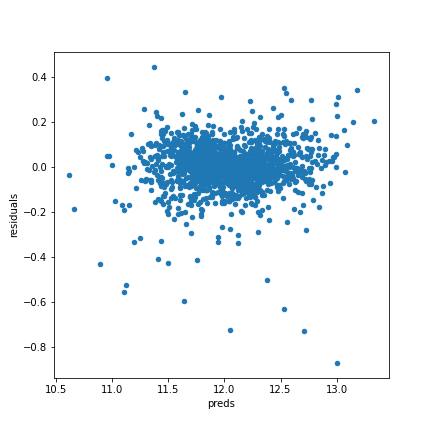
\includegraphics[width=7cm]{images/residual.png}
    \caption{Data residual}
    \label{fig:residual}
\end{figure}

We investigate the value distribution and correlation of SalePrice for each variable and introduce many new variables. For example, Figure [\ref{fig: price}] shows log transformation SalePrice distribution for each neighborhood. There are significantly different SalePrices among different neighborhoods. Details of feature engineering are listed in the following paragraphs.

These variables, which served as features of the dataset, were then used to predict the average price per square meter of each house.The next step was to investigate missing data. Variables with more than 50\% missing data would be removed from the dataset. Any observations which had missing values were also removed from the dataset. Below are a few feature engineering processes which were done to cleanse the dataset. 

Log transformation, in order to approximate normal distribution, log transformation has been applied for SalePrice, LotArea and LotFrontage etc. The Shapiro-Wilk test for normality is depicted in Fig. 2, in the left side, the log transformation of SalePrice distribution, while in right side it is SalePrice distribution. 

We transform the skewed numeric features by taking \(log(feature + 1)\) - this will make the features more normal. Create Dummy variables for the categorical features. Replace the numeric missing values (\emph{NaN's}\footnote{Not an Number}) with the mean of their respective columns. Finally, the residual of dataset was shown in Figure [\ref{fig:residual}]

\begin{figure}
    \centering
    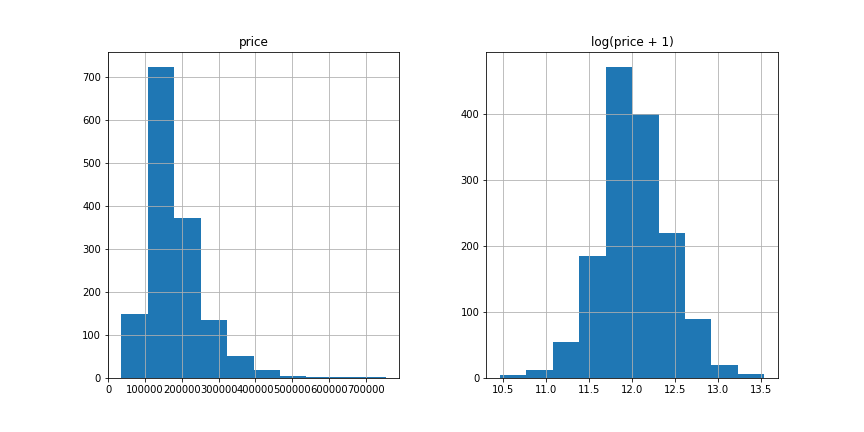
\includegraphics[width=7cm]{images/price.png}
    \caption{Log Sale Price}
    \label{fig: price}
\end{figure}

\subsection{Ridge Linear Regression}

Ridge regression there is one parameter alpha to choose for Ridge regression. Based on mean squared error scorer, we choose the alpha to get maximum score. Ridge regression give a penalty of L2 norm to the loss function, as follow:

\begin{equation}
\label{eq: ridge}
L = ||Y - X(\theta)||_2^2 - \alpha(||\theta||_2^2)\\
\end{equation}

When \(\alpha=0\), the penalty term has no effect, and the estimates produced by Ridge regression will be equal to Linear Regression. However, the impact of the shrinkage penalty grows, and the ridge regression coefficient estimates will approach zero. As can be seen, selecting a good value of \(\alpha\) is critical. Cross validation comes in handy for this purpose. The coefficient estimates produced by this method are also known as the L2 norm.

\subsection{Lasso Linear Regression}
 The Lasso model, as known as Least Absolute Shrinkage Selector Operator, is quite similar to ridge, but lets understand the difference them by implementing it in our big mart problem. Lasso model using L1 norm instead of L2 norm in the loss function, as follow:

\begin{equation}
\label{eq: lasso}
L = ||Y - X(\theta)||_2^2 - \alpha(||\theta||_2)\\
\end{equation}

This model is the same as the one above, but with a slight modification. Instead of penalty by L2 norm, this model uses the L1 one.

\subsection{Gradient Boosting}

XGBoost is short for eXtreme Gradient Boosting package. It is an efficient and scalable
implementation of gradient boosting framework by \citet{chen2016xgboost}.
The package includes efficient linear model solver and tree learning algorithm. It supports various
objective functions, including regression, classification and ranking. The package is made to be
extendible, so that users are also allowed to define their own objectives easily. 

\section{Experiments}

\subsection{Evaluation}

Kaggle evaluation standard is Root-Mean-Squared-Logarithmic-Error (RMSLE) between the logarithm of the predicted value and the logarithm of the observed sales price.

\begin{equation}
\label{eq: RMSLE}
RMSLE = \sqrt{\frac{1}{n}\sum_{t=1}^{n}(log(y_i+1) - log(\hat{y}_i+1))^2} \\
\end{equation}

Where \(y_i\) stands for \(log(SalePrice_i)\) and \(\hat{y}_i\) stands for
\(log(PredictSalePrice_i)\). The core part equates to \(log(SalePricei/PredictSalePricei)\). Using prediction SalePrice ratio could avoid the heavy weight age for expensive houses. In other words, prediction of cheap house prices is more important here. Kaggle house prices competition Public Leaderboard only shows the score for half of test data, it could avoid overfitting by many times of tries. Since prediction results need to be verified via Kaggle website to get the test score, and there is a limitation of no of submission per day, only selected test results are submitted. 

\subsection{Results}

\begin{table}
\centering
\begin{tabular}{lrl}
\hline \textbf{Method} & \textbf{RMSLE} \\ \hline
 Ridge & 0.13042 \\
 Lasso & 0.12455  \\
 XGBoost & 0.13278 \\
 Hybrid & \textbf{0.12342}  \\
\hline
\end{tabular}
\caption{\label{font-table} Comparasion of RMSLE. }
\label{table: rmsle}
\end{table}

After applying Ridge model to real estate price prediction, we obtained the result as shown in Figure [\ref{fig:ridge}]. Then we did the same with Lasso model, the results performed better (Figure [\ref{fig:lasso}]). For the best results, we aggregate them into a hybrid model between Ridge and Lasso as follow equation:

\begin{equation}
    \label{eq: hybrid}
    H = 0.5*Ridge + 0.5*Lasso
\end{equation}

as the following update equation


\begin{equation}
\label{eq: lasso}
L = ||Y - X(\theta)||_2^2 - 0.5*\alpha(||\theta||_2)\\ - 0.5*\alpha(||\theta||_2)\\
\end{equation}


\begin{figure}
    \centering
    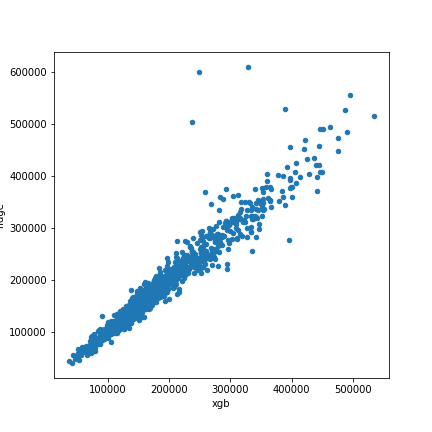
\includegraphics[width=7cm]{images/ridge.png}
    \caption{Ridge Prediction}
    \label{fig:ridge}
\end{figure}

\begin{figure}
    \centering
    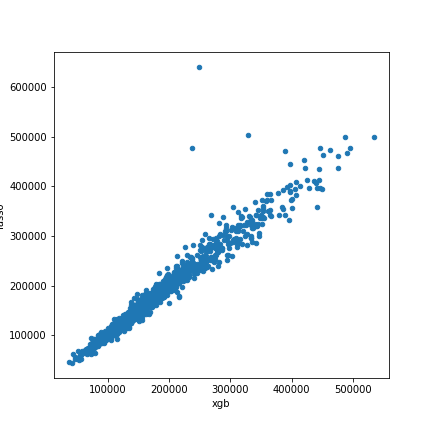
\includegraphics[width=7cm]{images/lasso.png}
    \caption{Lasso Prediction}
    \label{fig:lasso}
\end{figure}

\begin{figure}
    \centering
    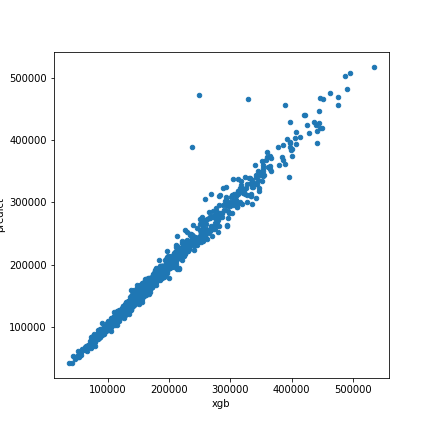
\includegraphics[width=7cm]{images/predict.png}
    \caption{Ridge combine with Lasso Prediction}
    \label{fig:predict}
\end{figure}


Comparative result of each model was shown on Table [\ref{table: rmsle}]. The hybrid model of Ridge, Lasso and XGB achieved the highest results in all models with minimum RMSLE value, 0.12342

The data distribution of three models, Ridge, Lasso and Hybrid , are shown on Figure [\ref{fig:ridge}], Figure [\ref{fig:lasso}], Figure [\ref{fig:predict}] respectively.

\section{Conclusion}

The test result indicates the usefulness of creating more new features. For those missing values the program needs to generate default values with different methods statistically. For example, mode method, noValue, zero value or median value.  There are a lot of key variables that affect house prices. If data are available ,a good idea is to introduce more features, for example income, salary, population, local amenities, cost of living, annual property tax, school, crime, marketing data.

Furthermore, Neural Networks are state-of-the-art models; it may help to improve prediction accuracy. We plan to build a Neural Network model to detect and predict house prices in Vietnamese, specially in Hanoi.

\section*{Acknowledgements}

The authors wish to thank Assoc. Prof. PHAM Van Hai for his reviews and encouragements; thank \cite{kaggle} to organise this greatful competition; thank \citet{de2011ames} for the dataset of Ames House Price.





% \section{Credits}

% This document has been adapted by Steven Bethard, Ryan Cotterrell and Rui Yan
% from the instructions for earlier ACL and NAACL proceedings, including those for 
% ACL 2019 by Douwe Kiela and Ivan Vuli\'{c},
% NAACL 2019 by Stephanie Lukin and Alla Roskovskaya, 
% ACL 2018 by Shay Cohen, Kevin Gimpel, and Wei Lu, 
% NAACL 2018 by Margaret Michell and Stephanie Lukin,
% 2017/2018 (NA)ACL bibtex suggestions from Jason Eisner,
% ACL 2017 by Dan Gildea and Min-Yen Kan, 
% NAACL 2017 by Margaret Mitchell, 
% ACL 2012 by Maggie Li and Michael White, 
% ACL 2010 by Jing-Shing Chang and Philipp Koehn, 
% ACL 2008 by Johanna D. Moore, Simone Teufel, James Allan, and Sadaoki Furui, 
% ACL 2005 by Hwee Tou Ng and Kemal Oflazer, 
% ACL 2002 by Eugene Charniak and Dekang Lin, 
% and earlier ACL and EACL formats written by several people, including
% John Chen, Henry S. Thompson and Donald Walker.
% Additional elements were taken from the formatting instructions of the \emph{International Joint Conference on Artificial Intelligence} and the \emph{Conference on Computer Vision and Pattern Recognition}.

% \section{Introduction}

% The following instructions are directed to authors of papers submitted to VLSP 2020 or accepted for publication in its proceedings.
% All authors are required to adhere to these specifications.
% Authors are required to provide a Portable Document Format (PDF) version of their papers.
% \textbf{The proceedings are designed for printing on A4 paper.}


% \section{Electronically-available resources}

% ACL provides this description and accompanying style files at
% \begin{quote}
% \url{https://vlsp.org.vn/resources/vlsp2020-latex-templates.zip}
% \end{quote}
% We strongly recommend the use of these style files, which have been appropriately tailored for the VLSP 2020 proceedings.

% \paragraph{\LaTeX-specific details:}
% The templates include the \LaTeX2e{} source (\texttt{\small acl2020.tex}),
% the \LaTeX2e{} style file used to format it (\texttt{\small acl2020.sty}),
% an ACL bibliography style (\texttt{\small acl\_natbib.bst}),
% an example bibliography (\texttt{\small acl2020.bib}),
% and the bibliography for the ACL Anthology (\texttt{\small anthology.bib}).


% \section{Length of Submission}
% \label{sec:length}

% The conference accepts submissions of long papers and short papers.
% Long papers may consist of up to eight (8) pages of content plus unlimited pages for references.
% Upon acceptance, final versions of long papers will be given one additional page -- up to nine (9) pages of content plus unlimited pages for references -- so that reviewers' comments can be taken into account.
% Short papers may consist of up to four (4) pages of content, plus unlimited pages for references.
% Upon acceptance, short papers will be given five (5) pages in the proceedings and unlimited pages for references. 
% For both long and short papers, all illustrations and tables that are part of the main text must be accommodated within these page limits, observing the formatting instructions given in the present document.
% Papers that do not conform to the specified length and formatting requirements are subject to be rejected without review.

% The conference encourages the submission of additional material that is relevant to the reviewers but not an integral part of the paper.
% There are two such types of material: appendices, which can be read, and non-readable supplementary materials, often data or code.
% Additional material must be submitted as separate files, and must adhere to the same anonymity guidelines as the main paper.
% The paper must be self-contained: it is optional for reviewers to look at the supplementary material.
% Papers should not refer, for further detail, to documents, code or data resources that are not available to the reviewers.
% Refer to Appendices~\ref{sec:appendix} and \ref{sec:supplemental} for further information. 

% Workshop chairs may have different rules for allowed length and whether supplemental material is welcome.
% As always, the respective call for papers is the authoritative source.


% \section{Anonymity}
% As reviewing will be double-blind, papers submitted for review should not include any author information (such as names or affiliations). Furthermore, self-references that reveal the author's identity, \emph{e.g.},
% \begin{quote}
% We previously showed \citep{Gusfield:97} \ldots
% \end{quote}
% should be avoided. Instead, use citations such as 
% \begin{quote}
% \citet{Gusfield:97} previously showed\ldots
% \end{quote}
% Please do not use anonymous citations and do not include acknowledgements.
% \textbf{Papers that do not conform to these requirements may be rejected without review.}

% Any preliminary non-archival versions of submitted papers should be listed in the submission form but not in the review version of the paper.
% Reviewers are generally aware that authors may present preliminary versions of their work in other venues, but will not be provided the list of previous presentations from the submission form.

% Once a paper has been accepted to the conference, the camera-ready version of the paper should include the author's names and affiliations, and is allowed to use self-references.

% \paragraph{\LaTeX-specific details:}
% For an anonymized submission, ensure that {\small\verb|\aclfinalcopy|} at the top of this document is commented out, and that you have filled in the paper ID number (assigned during the submission process on softconf) where {\small\verb|***|} appears in the {\small\verb|\def\aclpaperid{***}|} definition at the top of this document.
% For a camera-ready submission, ensure that {\small\verb|\aclfinalcopy|} at the top of this document is not commented out.


% \section{Multiple Submission Policy}
% Papers that have been or will be submitted to other meetings or publications must indicate this at submission time in the START submission form, and must be withdrawn from the other venues if accepted by ACL 2020. Authors of papers accepted for presentation at ACL 2020 must notify the program chairs by the camera-ready deadline as to whether the paper will be presented. We will not accept for publication or presentation the papers that overlap significantly in content or results with papers that will be (or have been) published elsewhere.

% Authors submitting more than one paper to VLSP 2020 must ensure that submissions do not overlap significantly (>25\%) with each other in content or results.



% \section{Formatting Instructions}

% Manuscripts must be in two-column format.
% Exceptions to the two-column format include the title, authors' names and complete addresses, which must be centered at the top of the first page, and any full-width figures or tables (see the guidelines in Section~\ref{ssec:title-authors}).
% \textbf{Type single-spaced.}
% Start all pages directly under the top margin.
% The manuscript should be printed single-sided and its length should not exceed the maximum page limit described in Section~\ref{sec:length}.
% Pages should be numbered in the version submitted for review, but \textbf{pages should not be numbered in the camera-ready version}.

% \paragraph{\LaTeX-specific details:}
% The style files will generate page numbers when {\small\verb|\aclfinalcopy|} is commented out, and remove them otherwise.


% \subsection{File Format}
% \label{sect:pdf}

% For the production of the electronic manuscript you must use Adobe's Portable Document Format (PDF).
% Please make sure that your PDF file includes all the necessary fonts (especially tree diagrams, symbols, and fonts with Asian characters).
% When you print or create the PDF file, there is usually an option in your printer setup to include none, all or just non-standard fonts.
% Please make sure that you select the option of including ALL the fonts.
% \textbf{Before sending it, test your PDF by printing it from a computer different from the one where it was created.}
% Moreover, some word processors may generate very large PDF files, where each page is rendered as an image.
% Such images may reproduce poorly.
% In this case, try alternative ways to obtain the PDF.
% One way on some systems is to install a driver for a postscript printer, send your document to the printer specifying ``Output to a file'', then convert the file to PDF.

% It is of utmost importance to specify the \textbf{A4 format} (21 cm x 29.7 cm) when formatting the paper.
% Print-outs of the PDF file on A4 paper should be identical to the hardcopy version.
% If you cannot meet the above requirements about the production of your electronic submission, please contact the publication chairs as soon as possible.

% \paragraph{\LaTeX-specific details:}
% PDF files are usually produced from \LaTeX{} using the \texttt{\small pdflatex} command.
% If your version of \LaTeX{} produces Postscript files, \texttt{\small ps2pdf} or \texttt{\small dvipdf} can convert these to PDF.
% To ensure A4 format in \LaTeX, use the command {\small\verb|\special{papersize=210mm,297mm}|}
% in the \LaTeX{} preamble (below the {\small\verb|\usepackage|} commands) and use \texttt{\small dvipdf} and/or \texttt{\small pdflatex}; or specify \texttt{\small -t a4} when working with \texttt{\small dvips}.

% \subsection{Layout}
% \label{ssec:layout}

% Format manuscripts two columns to a page, in the manner these
% instructions are formatted.
% The exact dimensions for a page on A4 paper are:

% \begin{itemize}
% \item Left and right margins: 2.5 cm
% \item Top margin: 2.5 cm
% \item Bottom margin: 2.5 cm
% \item Column width: 7.7 cm
% \item Column height: 24.7 cm
% \item Gap between columns: 0.6 cm
% \end{itemize}

% \noindent Papers should not be submitted on any other paper size.
% If you cannot meet the above requirements about the production of your electronic submission, please contact the publication chairs above as soon as possible.

% \subsection{Fonts}

% For reasons of uniformity, Adobe's \textbf{Times Roman} font should be used.
% If Times Roman is unavailable, you may use Times New Roman or \textbf{Computer Modern Roman}.

% Table~\ref{font-table} specifies what font sizes and styles must be used for each type of text in the manuscript.

% \begin{table}
% \centering
% \begin{tabular}{lrl}
% \hline \textbf{Type of Text} & \textbf{Font Size} & \textbf{Style} \\ \hline
% paper title & 15 pt & bold \\
% author names & 12 pt & bold \\
% author affiliation & 12 pt & \\
% the word ``Abstract'' & 12 pt & bold \\
% section titles & 12 pt & bold \\
% subsection titles & 11 pt & bold \\
% document text & 11 pt  &\\
% captions & 10 pt & \\
% abstract text & 10 pt & \\
% bibliography & 10 pt & \\
% footnotes & 9 pt & \\
% \hline
% \end{tabular}
% \caption{\label{font-table} Font guide. }
% \end{table}

% \paragraph{\LaTeX-specific details:}
% To use Times Roman in \LaTeX2e{}, put the following in the preamble:
% \begin{quote}
% \small
% \begin{verbatim}
% \usepackage{times}
% \usepackage{latexsym}
% \end{verbatim}
% \end{quote}


% \subsection{Ruler}
% A printed ruler (line numbers in the left and right margins of the article) should be presented in the version submitted for review, so that reviewers may comment on particular lines in the paper without circumlocution.
% The presence or absence of the ruler should not change the appearance of any other content on the page.
% The camera ready copy should not contain a ruler.

% \paragraph{Reviewers:}
% note that the ruler measurements may not align well with lines in the paper -- this turns out to be very difficult to do well when the paper contains many figures and equations, and, when done, looks ugly.
% In most cases one would expect that the approximate location will be adequate, although you can also use fractional references (\emph{e.g.}, this line ends at mark $295.5$).

% \paragraph{\LaTeX-specific details:}
% The style files will generate the ruler when {\small\verb|\aclfinalcopy|} is commented out, and remove it otherwise.

% \subsection{Title and Authors}
% \label{ssec:title-authors}

% Center the title, author's name(s) and affiliation(s) across both columns.
% Do not use footnotes for affiliations.
% Place the title centered at the top of the first page, in a 15-point bold font.
% Long titles should be typed on two lines without a blank line intervening.
% Put the title 2.5 cm from the top of the page, followed by a blank line, then the author's names(s), and the affiliation on the following line.
% Do not use only initials for given names (middle initials are allowed).
% Do not format surnames in all capitals (\emph{e.g.}, use ``Mitchell'' not ``MITCHELL'').
% Do not format title and section headings in all capitals except for proper names (such as ``BLEU'') that are
% conventionally in all capitals.
% The affiliation should contain the author's complete address, and if possible, an electronic mail address.

% The title, author names and addresses should be completely identical to those entered to the electronical paper submission website in order to maintain the consistency of author information among all publications of the conference.
% If they are different, the publication chairs may resolve the difference without consulting with you; so it is in your own interest to double-check that the information is consistent.

% Start the body of the first page 7.5 cm from the top of the page.
% \textbf{Even in the anonymous version of the paper, you should maintain space for names and addresses so that they will fit in the final (accepted) version.}


% \subsection{Abstract}
% Use two-column format when you begin the abstract.
% Type the abstract at the beginning of the first column.
% The width of the abstract text should be smaller than the
% width of the columns for the text in the body of the paper by 0.6 cm on each side.
% Center the word \textbf{Abstract} in a 12 point bold font above the body of the abstract.
% The abstract should be a concise summary of the general thesis and conclusions of the paper.
% It should be no longer than 200 words.
% The abstract text should be in 10 point font.

% \subsection{Text}
% Begin typing the main body of the text immediately after the abstract, observing the two-column format as shown in the present document.

% Indent 0.4 cm when starting a new paragraph.

% \subsection{Sections}

% Format section and subsection headings in the style shown on the present document.
% Use numbered sections (Arabic numerals) to facilitate cross references.
% Number subsections with the section number and the subsection number separated by a dot, in Arabic numerals.

% \subsection{Footnotes}
% Put footnotes at the bottom of the page and use 9 point font.
% They may be numbered or referred to by asterisks or other symbols.\footnote{This is how a footnote should appear.}
% Footnotes should be separated from the text by a line.\footnote{Note the line separating the footnotes from the text.}

% \subsection{Graphics}

% Place figures, tables, and photographs in the paper near where they are first discussed, rather than at the end, if possible.
% Wide illustrations may run across both columns.
% Color is allowed, but adhere to Section~\ref{ssec:accessibility}'s guidelines on accessibility.

% \paragraph{Captions:}
% Provide a caption for every illustration; number each one sequentially in the form:
% ``Figure 1. Caption of the Figure.''
% ``Table 1. Caption of the Table.''
% Type the captions of the figures and tables below the body, using 10 point text.
% Captions should be placed below illustrations.
% Captions that are one line are centered (see Table~\ref{font-table}).
% Captions longer than one line are left-aligned (see Table~\ref{tab:accents}).

% \begin{table}
% \centering
% \begin{tabular}{lc}
% \hline
% \textbf{Command} & \textbf{Output}\\
% \hline
% \verb|{\"a}| & {\"a} \\
% \verb|{\^e}| & {\^e} \\
% \verb|{\`i}| & {\`i} \\ 
% \verb|{\.I}| & {\.I} \\ 
% \verb|{\o}| & {\o} \\
% \verb|{\'u}| & {\'u}  \\ 
% \verb|{\aa}| & {\aa}  \\\hline
% \end{tabular}
% \begin{tabular}{lc}
% \hline
% \textbf{Command} & \textbf{Output}\\
% \hline
% \verb|{\c c}| & {\c c} \\ 
% \verb|{\u g}| & {\u g} \\ 
% \verb|{\l}| & {\l} \\ 
% \verb|{\~n}| & {\~n} \\ 
% \verb|{\H o}| & {\H o} \\ 
% \verb|{\v r}| & {\v r} \\ 
% \verb|{\ss}| & {\ss} \\
% \hline
% \end{tabular}
% \caption{Example commands for accented characters, to be used in, \emph{e.g.}, \BibTeX\ names.}\label{tab:accents}
% \end{table}

% \paragraph{\LaTeX-specific details:}
% The style files are compatible with the caption and subcaption packages; do not add optional arguments.
% \textbf{Do not override the default caption sizes.}


% \subsection{Hyperlinks}
% Within-document and external hyperlinks are indicated with Dark Blue text, Color Hex \#000099.

% \subsection{Citations}
% Citations within the text appear in parentheses as~\citep{Gusfield:97} or, if the author's name appears in the text itself, as \citet{Gusfield:97}.
% Append lowercase letters to the year in cases of ambiguities.  
% Treat double authors as in~\citep{Aho:72}, but write as in~\citep{Chandra:81} when more than two authors are involved. Collapse multiple citations as in~\citep{Gusfield:97,Aho:72}. 

% Refrain from using full citations as sentence constituents.
% Instead of
% \begin{quote}
%   ``\citep{Gusfield:97} showed that ...''
% \end{quote}
% write
% \begin{quote}
% ``\citet{Gusfield:97} showed that ...''
% \end{quote}

% \begin{table*}
% \centering
% \begin{tabular}{lll}
% \hline
% \textbf{Output} & \textbf{natbib command} & \textbf{Old ACL-style command}\\
% \hline
% \citep{Gusfield:97} & \small\verb|\citep| & \small\verb|\cite| \\
% \citealp{Gusfield:97} & \small\verb|\citealp| & no equivalent \\
% \citet{Gusfield:97} & \small\verb|\citet| & \small\verb|\newcite| \\
% \citeyearpar{Gusfield:97} & \small\verb|\citeyearpar| & \small\verb|\shortcite| \\
% \hline
% \end{tabular}
% \caption{\label{citation-guide}
% Citation commands supported by the style file.
% The style is based on the natbib package and supports all natbib citation commands.
% It also supports commands defined in previous ACL style files for compatibility.
% }
% \end{table*}

% \paragraph{\LaTeX-specific details:}
% Table~\ref{citation-guide} shows the syntax supported by the style files.
% We encourage you to use the natbib styles.
% You can use the command {\small\verb|\citet|} (cite in text) to get ``author (year)'' citations as in \citet{Gusfield:97}.
% You can use the command {\small\verb|\citep|} (cite in parentheses) to get ``(author, year)'' citations as in \citep{Gusfield:97}.
% You can use the command {\small\verb|\citealp|} (alternative cite without  parentheses) to get ``author year'' citations (which is useful for  using citations within parentheses, as in \citealp{Gusfield:97}).


% \subsection{References}
% Gather the full set of references together under the heading \textbf{References}; place the section before any Appendices. 
% Arrange the references alphabetically by first author, rather than by order of occurrence in the text.

% Provide as complete a citation as possible, using a consistent format, such as the one for \emph{Computational Linguistics\/} or the one in the  \emph{Publication Manual of the American 
% Psychological Association\/}~\citep{APA:83}.
% Use full names for authors, not just initials.

% Submissions should accurately reference prior and related work, including code and data.
% If a piece of prior work appeared in multiple venues, the version that appeared in a refereed, archival venue should be referenced.
% If multiple versions of a piece of prior work exist, the one used by the authors should be referenced.
% Authors should not rely on automated citation indices to provide accurate references for prior and related work.

% The following text cites various types of articles so that the references section of the present document will include them.
% \begin{itemize}
% \item Example article in journal: \citep{Ando2005}.
% \item Example article in proceedings, with location: \citep{borschinger-johnson-2011-particle}.
% \item Example article in proceedings, without location: \citep{andrew2007scalable}.
% \item Example arxiv paper: \citep{rasooli-tetrault-2015}. 
% \end{itemize}


% \paragraph{\LaTeX-specific details:}
% The \LaTeX{} and Bib\TeX{} style files provided roughly follow the American Psychological Association format.
% If your own bib file is named \texttt{\small acl2020.bib}, then placing the following before any appendices in your \LaTeX{}  file will generate the references section for you:
% \begin{quote}\small
% \verb|\bibliographystyle{acl_natbib}|\\
% \verb|\bibliography{acl2020}|
% \end{quote}

% You can obtain the complete ACL Anthology as a Bib\TeX\ file from \url{https://aclweb.org/anthology/anthology.bib.gz}.
% To include both the anthology and your own bib file, use the following instead of the above.
% \begin{quote}\small
% \verb|\bibliographystyle{acl_natbib}|\\
% \verb|\bibliography{anthology,acl2020}|
% \end{quote}


% \subsection{Digital Object Identifiers}
% As part of our work to make ACL materials more widely used and cited outside of our discipline, ACL has registered as a CrossRef member, as a registrant of Digital Object Identifiers (DOIs), the standard for registering permanent URNs for referencing scholarly materials.

% All camera-ready references are required to contain the appropriate DOIs (or as a second resort, the hyperlinked ACL Anthology Identifier) to all cited works.
% Appropriate records should be found for most materials in the current ACL Anthology at \url{http://aclanthology.info/}.
% As examples, we cite \citep{goodman-etal-2016-noise} to show you how papers with a DOI will appear in the bibliography.
% We cite \citep{harper-2014-learning} to show how papers without a DOI but with an ACL Anthology Identifier will appear in the bibliography.

% \paragraph{\LaTeX-specific details:}
% Please ensure that you use Bib\TeX\ records that contain DOI or URLs for any of the ACL materials that you reference.
% If the Bib\TeX{} file contains DOI fields, the paper title in the references section will appear as a hyperlink to the DOI, using the hyperref \LaTeX{} package.


% \subsection{Appendices}
% Appendices, if any, directly follow the text and the
% references (but only in the camera-ready; see Appendix~\ref{sec:appendix}).
% Letter them in sequence and provide an informative title:
% \textbf{Appendix A. Title of Appendix}.

% \section{Accessibility}
% \label{ssec:accessibility}

% In an effort to accommodate people who are color-blind (as well as those printing to paper), grayscale readability is strongly encouraged.
% Color is not forbidden, but authors should ensure that tables and figures do not rely solely on color to convey critical distinctions.
% A simple criterion:
% All curves and points in your figures should be clearly distinguishable without color.

% \section{Translation of non-English Terms}

% It is also advised to supplement non-English characters and terms with appropriate transliterations and/or translations since not all readers understand all such characters and terms.
% Inline transliteration or translation can be represented in the order of:
% \begin{center}
% \begin{tabular}{c}
% original-form \\
% transliteration \\
% ``translation''
% \end{tabular}
% \end{center}

% \section{\LaTeX{} Compilation Issues}
% You may encounter the following error during compilation: 
% \begin{quote}
% {\small\verb|\pdfendlink|} ended up in different nesting level than {\small\verb|\pdfstartlink|}.
% \end{quote}
% This happens when \texttt{\small pdflatex} is used and a citation splits across a page boundary.
% To fix this, the style file contains a patch consisting of two lines:
% (1) {\small\verb|\RequirePackage{etoolbox}|} (line 455 in \texttt{\small acl2020.sty}), and
% (2) A long line below (line 456 in \texttt{\small acl2020.sty}).

% If you still encounter compilation issues even with the patch enabled, disable the patch by commenting the two lines, and then disable the \texttt{\small hyperref} package by loading the style file with the \texttt{\small nohyperref} option:

% \noindent
% {\small\verb|\usepackage[nohyperref]{acl2020}|}

% \noindent
% Then recompile, find the problematic citation, and rewrite the sentence containing the citation. (See, {\em e.g.}, \url{http://tug.org/errors.html})

% \section*{Acknowledgments}

% The acknowledgments should go immediately before the references. Do not number the acknowledgments section.
% Do not include this section when submitting your paper for review.

% \bibliography{anthology,acl2020}
% \bibliographystyle{acl_natbib}

% \appendix

% \section{Appendices}
% \label{sec:appendix}
% Appendices are material that can be read, and include lemmas, formulas, proofs, and tables that are not critical to the reading and understanding of the paper. 
% Appendices should be \textbf{uploaded as supplementary material} when submitting the paper for review.
% Upon acceptance, the appendices come after the references, as shown here.

% \paragraph{\LaTeX-specific details:}
% Use {\small\verb|\appendix|} before any appendix section to switch the section numbering over to letters.


% \section{Supplemental Material}
% \label{sec:supplemental}
% Submissions may include non-readable supplementary material used in the work and described in the paper.
% Any accompanying software and/or data should include licenses and documentation of research review as appropriate.
% Supplementary material may report preprocessing decisions, model parameters, and other details necessary for the replication of the experiments reported in the paper.
% Seemingly small preprocessing decisions can sometimes make a large difference in performance, so it is crucial to record such decisions to precisely characterize state-of-the-art methods. 

% Nonetheless, supplementary material should be supplementary (rather than central) to the paper.
% \textbf{Submissions that misuse the supplementary material may be rejected without review.}
% Supplementary material may include explanations or details of proofs or derivations that do not fit into the paper, lists of
% features or feature templates, sample inputs and outputs for a system, pseudo-code or source code, and data.
% (Source code and data should be separate uploads, rather than part of the paper).

% The paper should not rely on the supplementary material: while the paper may refer to and cite the supplementary material and the supplementary material will be available to the reviewers, they will not be asked to review the supplementary material.


\bibliography{anthology,acl2020}
\bibliographystyle{acl_natbib}

\end{document}
